\section{Introduction to the Reduced Model}
The aerolastic analysis is one of the costly operation in the optimization process, in fact many computation must be performed, with different software; to perform an aerolastic analysis a static structural analysis, an aerodynamic analysis and a dynamic structural analysis, for each iteration is required. So to contain the cost of the analysis models with a low computational cost are needed. In parallel with the multidisciplinary design optimization process, Josè Serralta and Dimitrios Glenis, work to the project which the objective is to perform a model reduction from a complex 3D geometry to a simpler one with a computational cost compatible with the one required for the optimization process and yet a sufficient accuracy for a satisfactory preliminary design, as is illustrated in their report \cite{bru}. A modal analysis will be performed on both the complete and the reduced model, to check that their dynamic are indeed similar. Then, the reduced model will be used for the static, dynamic and aeroelastic analysis in the optimization loop.\\
In the preliminary design phase simplified beams models, knowns as stick models, are used to perform static and dynamic aeroelastic analysis, to have some preliminary results without high cost. During the last stages of the design, high fidelity detailed 3D FEM models are used for design validation and optimization, but this kind of models are too expensive for the MDO process. Thus, condensed models are created for dynamic simulations, using reduction techniques to develop models which are sufficiently simple but sophisticated enough to predict the dynamic behavior \cite{bomb}. Guyan reduction technique was one of the first to appear, it is one of the most popular condensation methods and it is included in many commercial FEM codes \cite{ter}.
\subsection{Approach for the Reduced Model}
In Fig. \ref{fig:4_1} are showed the different modeling levels for a wing. As we can see the structure of the wing can be represented with a box-like model, where the semi-monocoque structure, composed by discrete stiffeners, like stringer, and thin walled panels, like the cover skin and ribs, is modeled and meshed using FEM elements, like beam and shell elements. Another approach to model the wing is using a beam-like model, where each beam element represent the stiffness properties of an associated wing strip. \\
In literature two approaches are considered:
\begin{itemize}
	\item Reduction techniques, such as guyan or IRS \cite{don}, can be used to reduce the original 3D FEM model with $N$ degree of freedom to one which a much smaller number of nodal points $M < < N$. The DoF of the reduced model are referred as masters, and the deleted ones as slaves. The selection of the master nodes is very important, although there exist iterative methods which make their selection much less critical \cite{qui}. The result of condensation is still a 3D model, but with less nodes.
	\item Generating a stick model by extracting the stiffness properties of the full 3D FEM model and applying them to a set of beam elements extending along the structure’s elastic axis \cite{ite}. In this case the full model is not reduced, but a new equivalent FEM model is built.
\end{itemize}
The reduction techniques are usually used for dynamic analysis, while for the aeroelastic studies the condensation to stick models is more used, so for this project the second approach is adopted.\\
So the main idea for the reduced model is to start from the detailed FEM model with the shell elements, perform an static analysis with exploration load, and from that analysis compute the stiffness and inertial properties of a section, then for each section one beam elements are associated to one section, and we set its stiffness and inertial properties the properties of the respective section.\\

\begin{figure}[H]
	\centering
	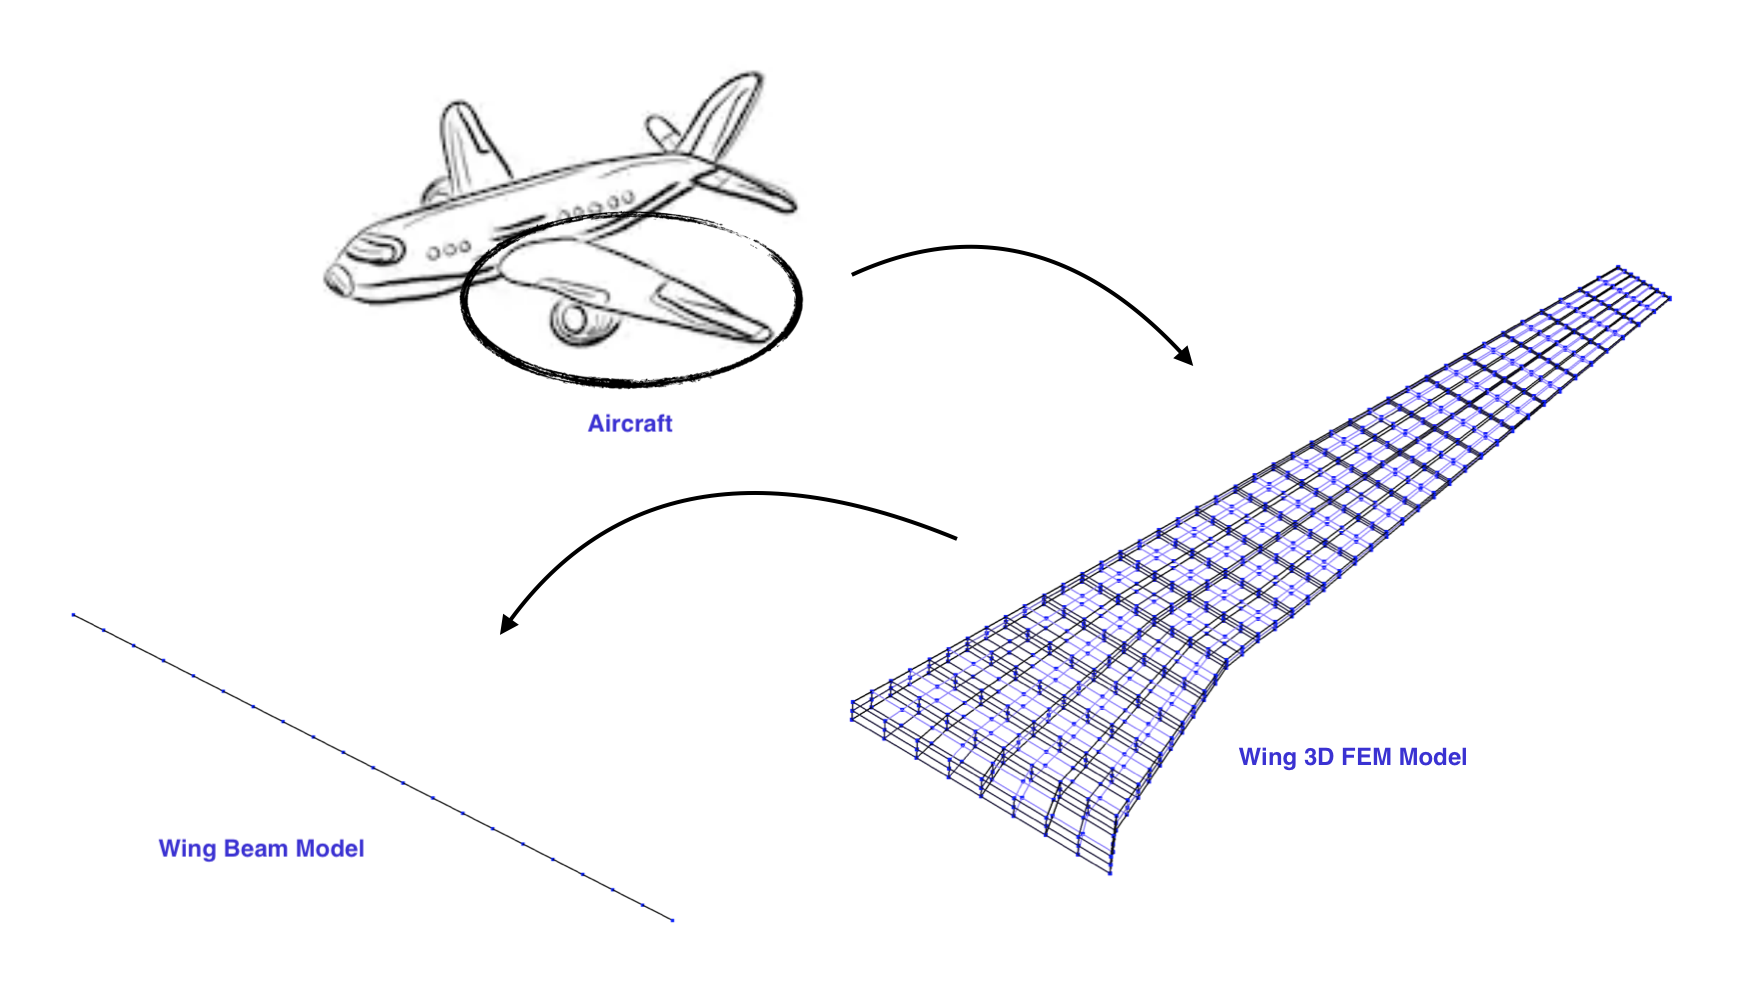
\includegraphics[width = 0.8\textwidth]{./Immagini/4_1.png}
	\caption{Different modeling levels }
	\label{fig:4_1}
\end{figure}
\section{Structure of the Code}
In this part we will see how the stick model is obtained from the full model, and how the validation of the stick model is performed. In Fig. \ref{fig:4_2} is represented the flow chart of the reduction model:
\begin{figure}[H]
	\centering
	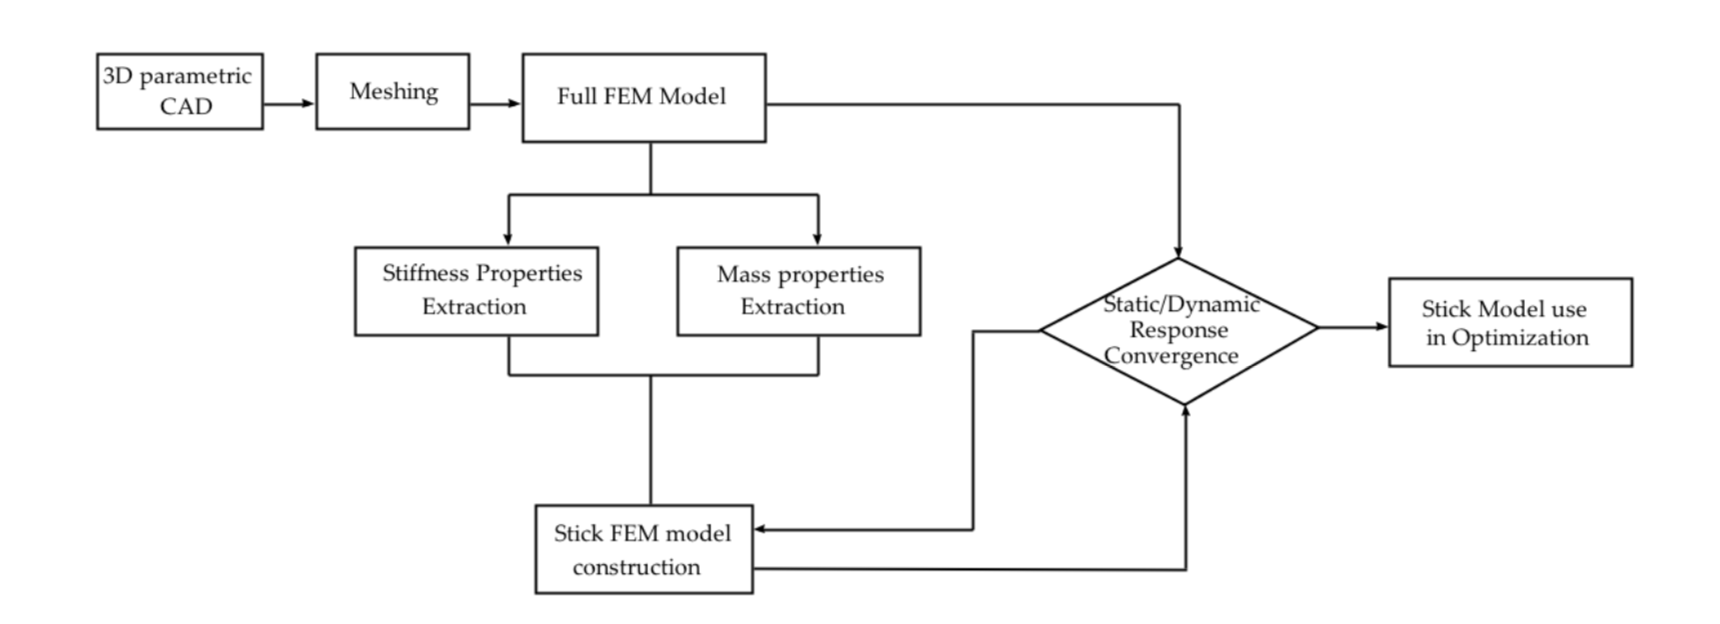
\includegraphics[width = 1\textwidth]{./Immagini/4_2.png}
	\caption{Flow chart of the reduced model code }
	\label{fig:4_2}
\end{figure}
The Full FEM model is created using the geometry component, that we discuss in the chapter 2. From the full FEM model the mass and stiffness properties of the section, which we split our model, are extracted using the Nastran Weight Generator instrument. Then the stick model be created, importing the mass and stiffness properties of each section in one beam element. The stick model need now to be validated, one static analysis and one modal analysis will be performed on the stick model, then the result will be compared to the result of the same analysis performed on the full model. While the results is not acceptable some corrective coefficient will be changed until the convergence of the relative error is guaranteed. When the stick model is validated, it can be used in the optimization code, in particular in the MDA loop, to obtain a gain on the computational cost of this operation.
\subsection{Creation of the FEM model}
To create the FEM model of the stick model the procedure it's the same of the creation of the FEM model of the full model. As we saw in the chapter 2, after the geometry component creates the \textit{.igs} file, and after the program gmsh create the FEM mesh, the structure component write the bfd file, putting the properties of each elements in a NASTRAN card, from a template \textit{.bdf} file. In this case we use another \textit{.bdf} template, where there are just BAR elements (the beam elements in the NASTRAN95 language). For this part just the number of the elements, equal to the number of the section used to split the full model, and the position of the nodes are required. For each element also a lumped mass will be created, and for the moment it's value is 0 and it's located in the first node of the element, when we will have the information about the mass propierties, using the offset command we will change the effective position of the lumped mass. At the end of this process we will have a \textit{.bdf file} of a stick model, that present $N$ BAR elements and $N$ lumped mass, but without information about the material and inertia properties. In Fig. \ref{fig:4_3} are schematized what this component do:
\begin{figure}[H]
	\centering
	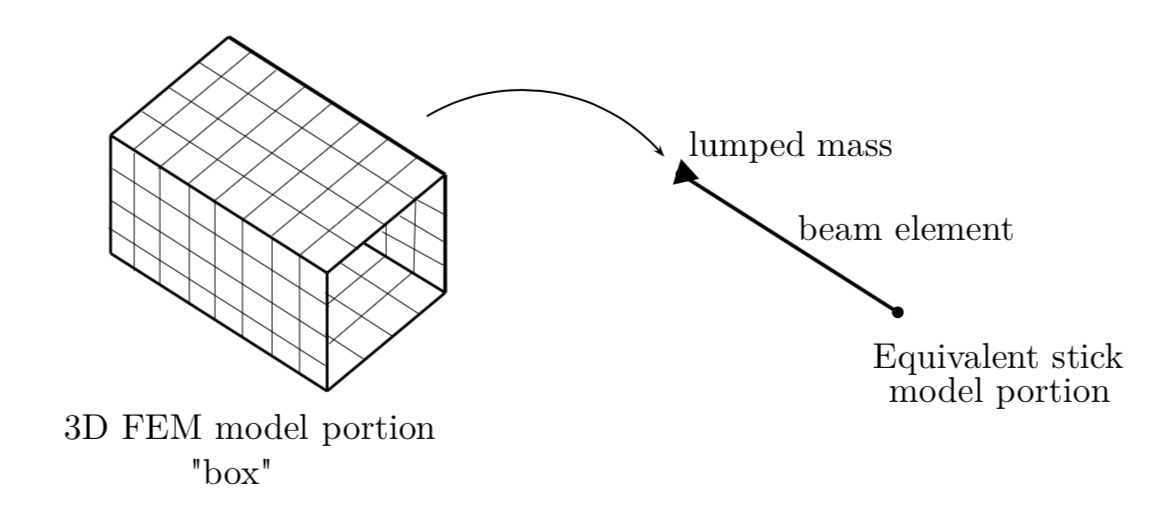
\includegraphics[width = 0.8\textwidth]{./Immagini/4_3.png}
	\caption{Schematization of the creation of the stick model }
	\label{fig:4_3}
\end{figure}
\subsection{Extraction of Stiffness and Inertia Properties}
Starting from the 3D FEM model of the structure, we split it into section called boxes, which could be delimited by the ribs of the wing. The object is to build a 1D model in which each box is represented from an equivalent beam element. To do this as first we need to determinate the stiffness properties ($A,I_y,I_z,J$) and the inertia properties ($m,x_G,I_G$) to give to the beam element so it's representative of the box. 
\subsubsection{Stiffness Properties}
The flexibility matrix \textbf{C} of each box is obtained from the displacements due to a set of unitary loads applied to one of its sections. \cite{bru}.
\begin{figure}[H]
	\centering
	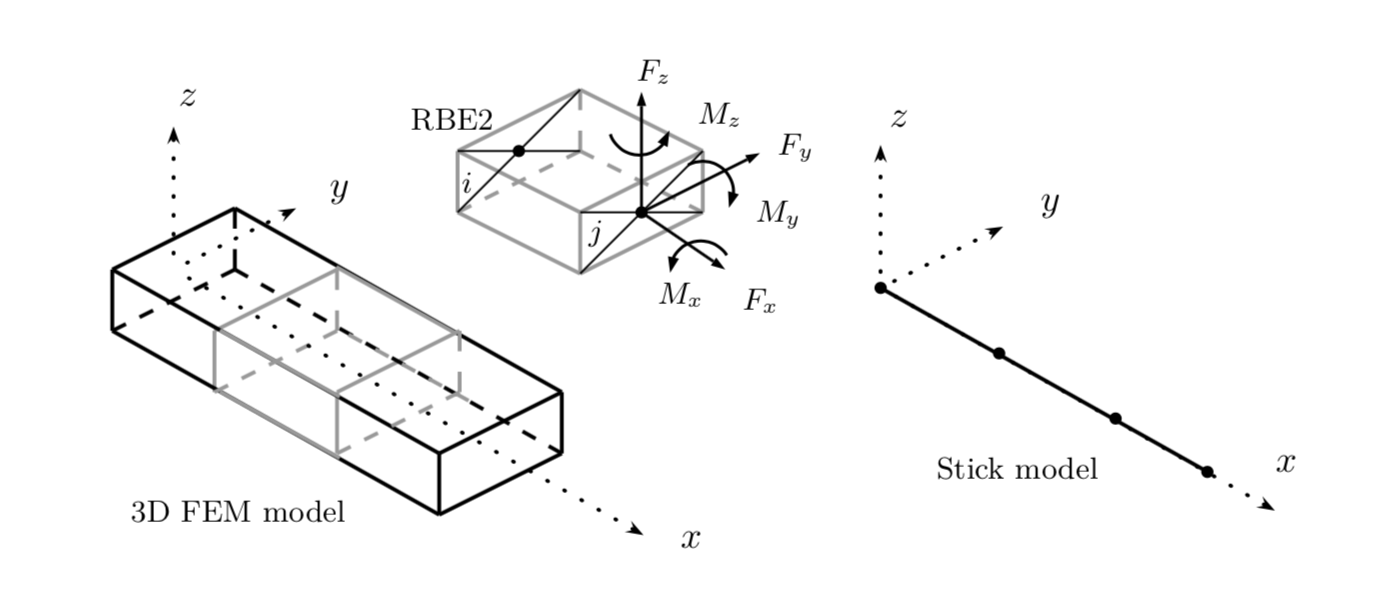
\includegraphics[width = 0.8\textwidth]{./Immagini/4_4.png}
	\caption{Detailed model subdivisions and unitary loads for the extraction}
	\label{fig:4_4}
\end{figure}
In Fig.\ref{fig:4_4} is showed a box with the 2 associated nodes of the reduced model (nodes \textit{i} and \textit{j}). To compute the flexibility matrix \textbf{C} a set of six unitary loads are applied at node \textit{j} and the consequent displacements are measured at nodes \textit{i} and \textit{j}. \\
Let $\mathbf{C_i}$ and $\mathbf{C_j}$ be the flexibility matrices relating loads at \textit{j} with displacements at \textit{i} and \textit{j} respectively. If a unitary load vector \textbf{F} is applied, then from $C\dot F = U$ the associated displacements \textit{u} provides a column of matrix \textbf{C}. In this way, with the displacements from the six unitary loads, the six columns of matrices $\mathbf{C_i}$ and $\mathbf{C_j}$ are built. \cite{bru}\\
The $\mathbf{C_i}$ and $\mathbf{C_j}$ are the flexibility matrices relating loads at node \textit{j} with displacement at nodes \textit{i} and \textit{j} respectively. We can obtain the flexibility matrix of the box from the forces and strains. Strains are approximated obtained from these relations:
\begin{equation*}
\epsilon_x=\frac{u_{x_j}-u_{x_i}}{\Delta x}; \qquad \gamma_y=\frac{u_{y_j}-u_{y_i}}{\Delta x}; \qquad \gamma_z=\frac{u_{z_j}-u_{z_i}}{\Delta x}
\end{equation*}
\begin{equation*}
\kappa_x=\frac{\theta_{x_j}-\theta_{x_i}}{\Delta x}; \qquad \gamma_y=\frac{\theta_{y_j}-\theta_{y_i}}{\Delta x}; \qquad \gamma_z=\frac{\theta_{z_j}-\theta_{z_i}}{\Delta x}
\end{equation*}
where $u_{x_j}$ is the displacement in \textit{x}-direction at node \textit{j}, $\theta_{x_j}$ is the rotation in \textit{x}-direction at node \textit{j}, and the same for the others, $\Delta x$ is the length of the box. So the flexibility matrix of the box will be:
\begin{equation*}
\mathbf{C}=\frac{\mathbf{C_j}-\mathbf{C_i}}{\Delta x}
\end{equation*}
from that we can obtain the stiffness matrix of the box from:
\begin{equation*}
\mathbf{K}=\mathbf{C^{-1}}
\end{equation*}
From the stiffness matric we can obtain the section proprieties, from the following relation:
\begin{equation*}
\begin{pmatrix}
F_x\\
F_y\\
F_z\\
M_x\\
M_y\\
M_z\\
\end{pmatrix} =
\begin{bmatrix}
A_{11}&0&0&0&A_{12}&A_{13}\\
0&S_{11}&S_{12}& S_{13}&0&0   \\
0&S_{21}&S_{22}& S_{23}&0&0   \\
0&S_{31}&S_{32}& S_{33}&0&0   \\
A_{21}&0&0&0&A_{22}&A_{23}\\
A_{31}&0&0&0&A_{32}&A_{33}\\
\end{bmatrix}
\begin{pmatrix}
\epsilon_x \\
\gamma_y \\
\gamma_z \\
\kappa_x \\
\kappa_y \\
\kappa_z 
\end{pmatrix}
\end{equation*}
Where $A_{ij}$ and $S_{ij}$ are the stiffness terms associated to axial and shear sets. So from the constitutive equation it's possible to determinate the section properties:
\begin{equation*}
\mathbf{A} =
\begin{bmatrix}
A_{11}&0&0\\
&A_{22}&0\\
sym&&A_{33}
\end{bmatrix}=
\begin{bmatrix}
EA&0&0\\
&EI_y&0\\
sym&&EI_z
\end{bmatrix}
\end{equation*}
\begin{equation*}
\mathbf{S} =
\begin{bmatrix}
S_{11}&0&0\\
&S_{22}&0\\
sym&&S_{33}
\end{bmatrix}=
\begin{bmatrix}
GA_y&0&0\\
&GA_z&0\\
sym&&GJ
\end{bmatrix}
\end{equation*}
From this it's possible to extract the section properties $A,I_y,I_z,J$ to give to the beam element to be representative of the box section.
\subsubsection{Inertia Properties}
The inertia properties of each box are extracted using the \textit{NASTRAN grid point weight generator} \cite{msc}, which generate an output file containing the information relative to the position of the center of gravity $X_G$, the mass $m$ and inertias $I$ of the box. In Fig. \ref{fig:4_5} is showed an example of the output file. From this information we will change the position and the properties of the lumped mass that we create in the first phase. Since the mass of the boxes are represented from the lumped mass, the density of the material is set to 0.
\begin{figure}[H]
	\centering
	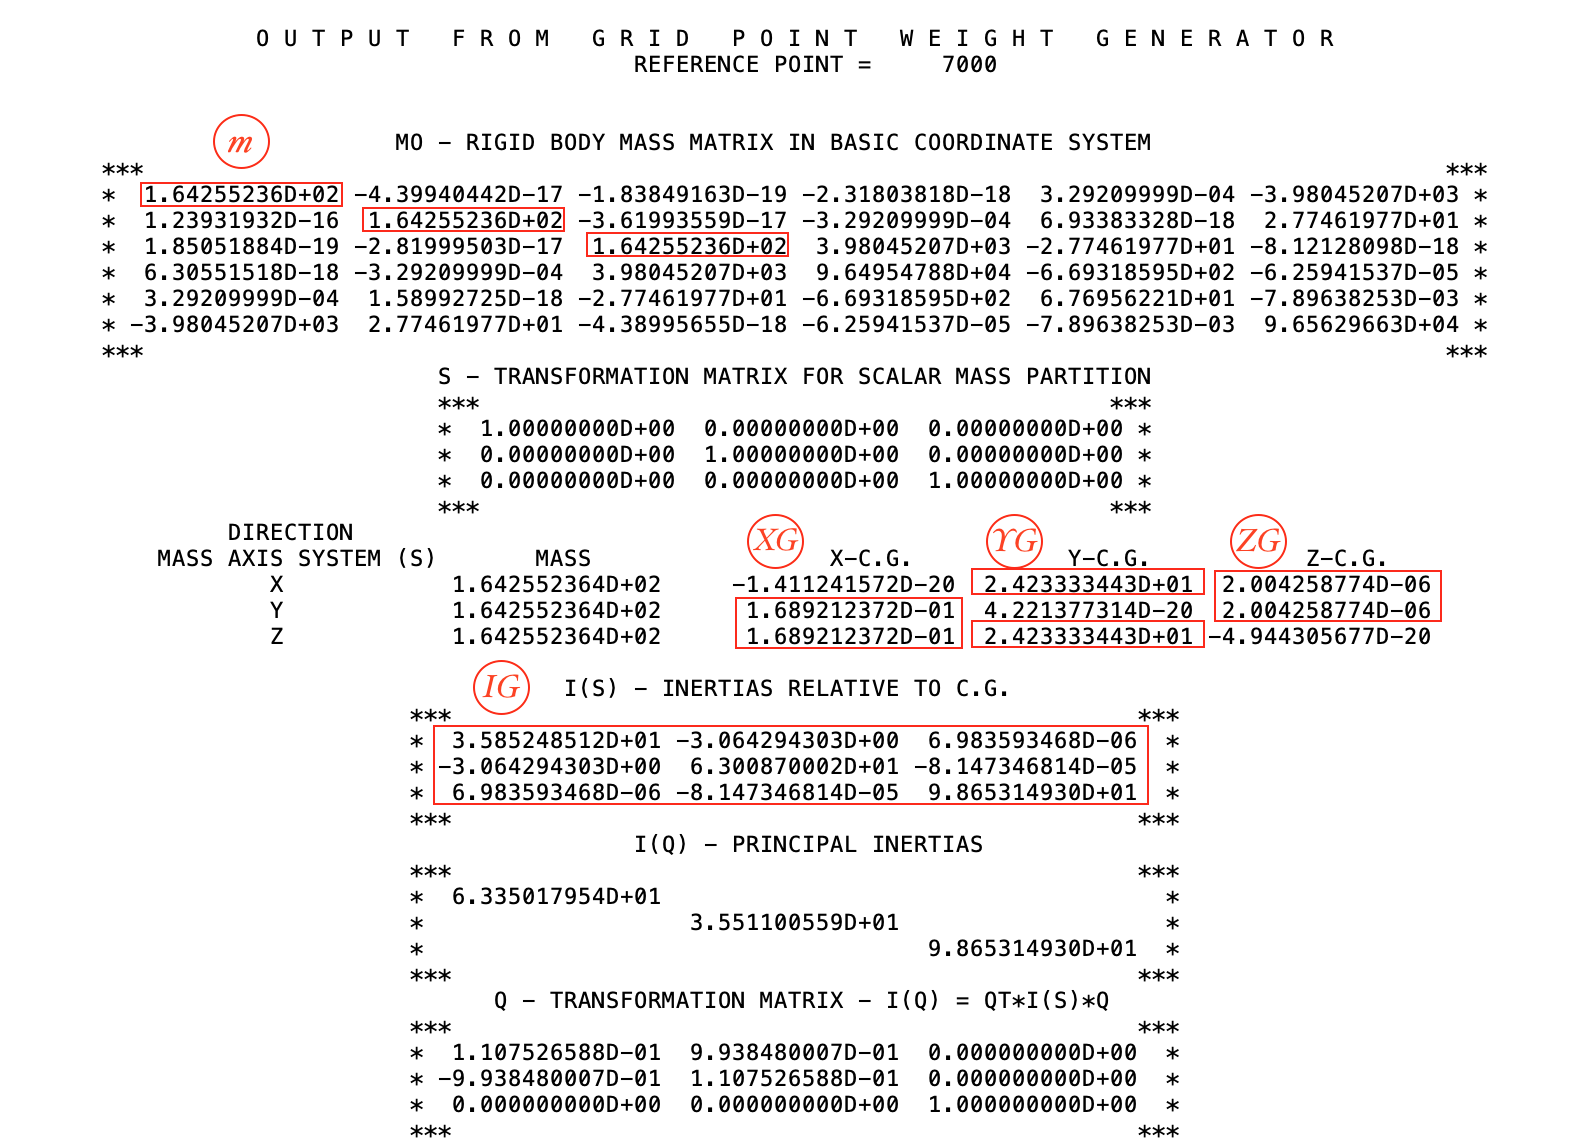
\includegraphics[width = 1\textwidth]{./Immagini/4_5.png}
	\caption{NASTRAN grid point weight generator output file}
	\label{fig:4_5}
\end{figure}
At the end of the process the beam element has the stiffness and inertia properties of the box, as the Fig. \ref{fig:4_6} shows:
\begin{figure}[H]
	\centering
	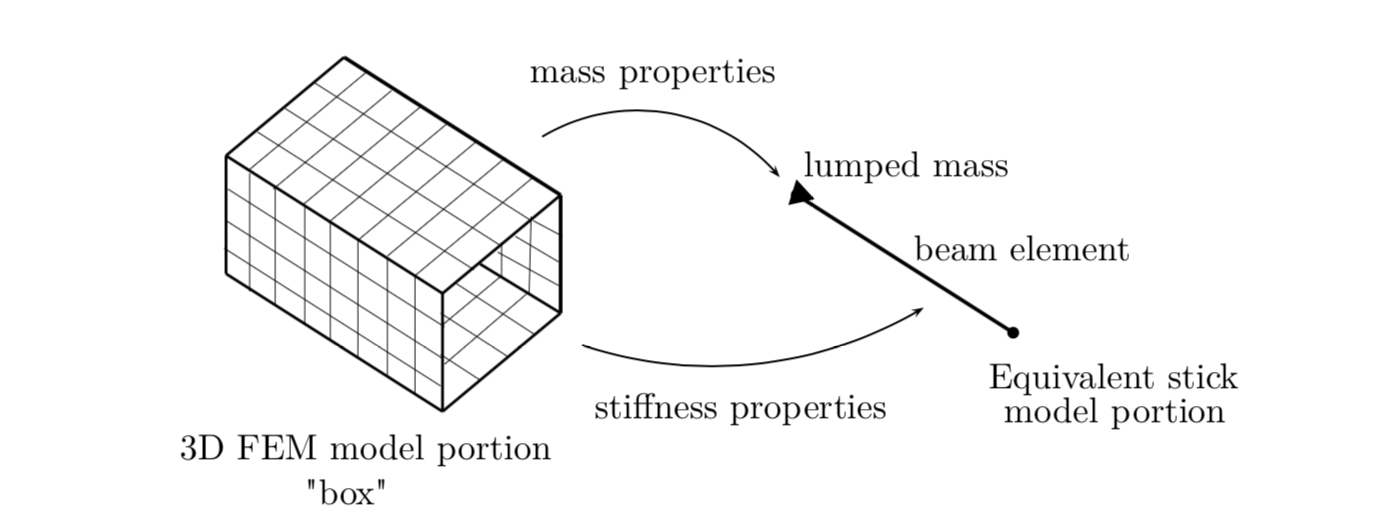
\includegraphics[width = 1\textwidth]{./Immagini/4_6.png}
	\caption{Schematization of the creation of the stick model and importing of the properties}
	\label{fig:4_6}
\end{figure}
\section{Validation of the Stick Model}
For the validation of the stick model two comparison have been done, one on the static response results, in terms of displacement and rotation of the nodes, and one on the modal analysis, in terms of natural frequencies and modal shapes. In both the cases to allow the comparison, since the number of nodes and their position is different, a series of nodes have been added in the full model, in particular we add in the full model the same nodes used for the stick model in the same relative position, then we connected these nodes to the structural nodes of the full model between rigid connection. In that way we can comparison the displacement, the eigenvector and the eigenvalue of the two different models.
\subsection{Comparison of the Static Response}
To do the comparison of the static response an exploration load have been applied at the wing tip. To determinate the displacements and the rotation in all the direction 6 different load have been applied, 3 force of 1 $N$ applied on the $x, y$ and $z$ direction, $F_x,F_y$ and $F_z$, and 3 moments of 1 $N\ mm$, $;M_x,M_y$ and $M_z$.\\
In the Fig. \ref{fig:4_7} there are the results obtained from the comparison.\\
As we can see the errors on the displacements are $\approx 15\%$ at the wingtip, while the errors on the rotation are smaller, $\approx 10\%$, and $\approx 1\%$ on the horizontal rotation $\theta_y$. \\
\begin{figure}[H]
	\centering
	\subfigure[Longitudinal displacement $u_x$]{
			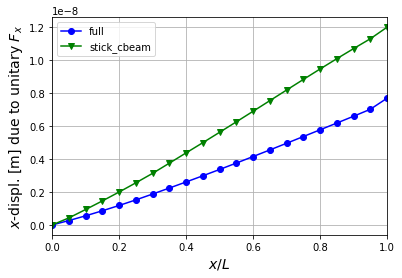
\includegraphics[width = 0.4\textwidth]{./Immagini/4_7.png}
		\label{fig:subfig1}
	}
	\subfigure[Torsional rotation $\theta_x$]{
		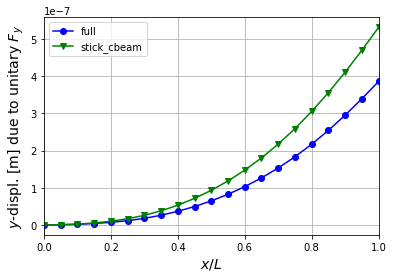
\includegraphics[width = 0.4\textwidth]{./Immagini/4_8.png}
		\label{fig:subfig2}
	}
	\subfigure[Horizontal displacement $u_y$]{
	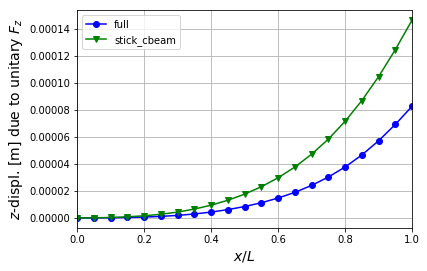
\includegraphics[width = 0.4\textwidth]{./Immagini/4_9.png}
	\label{fig:subfig1}
}
\subfigure[Horizontal rotation $\theta_y$]{
	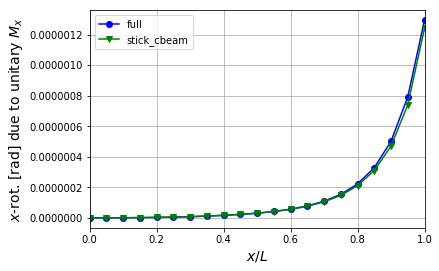
\includegraphics[width = 0.4\textwidth]{./Immagini/4_10.png}
	\label{fig:subfig2}
}
	\subfigure[Vertical displacement $u_z$]{
	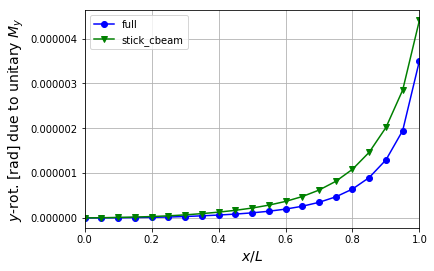
\includegraphics[width = 0.4\textwidth]{./Immagini/4_11.png}
	\label{fig:subfig1}
}
\subfigure[Vertical rotation $\theta_z$]{
	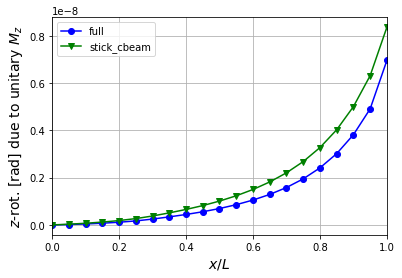
\includegraphics[width = 0.4\textwidth]{./Immagini/4_12.png}
	\label{fig:subfig2}
}
\caption[Optional caption for list of figures]{Comparison of the static response }
	\label{fig:4_7}
\end{figure}

To get better results it's possible to adopt a correction on the Young module $E$ and on the shear module $G$, using virtual modules obtained from the relative error on the displacements and rotation:
\begin{equation*}
E_{corr}=\frac{u_{z|stick}}{u_{z|full}}E;\qquad G_{corr}=\frac{\theta_{x|stick}}{\theta_{x|full}}G
\end{equation*}
\subsection{Comparison of the Modal Properties}
To do the comparison of the modal properties we compare as first the modal shapes of the two model, and after the natural frequencies. Also in this case the extra nodes are used in the full model to have a compatibility for the two modal shapes. To compare the modal shape the Modal Assurance Criterion \textbf{MAC} have been used.
\subsubsection{Modal Assurance Criterion MAC}
The function of the modal assurance criterion (MAC) is to provide a measure of consistency between estimates of a modal vector. \cite{mac2} The Modal Assurance Criterion is a vector correlation index frequently used in experimental dynamics to quantify the similarity of mode shapes\cite{mac}.\\
This criterion is based on the computation of a normalized scalar product of the eigenvector of the system given by:
\begin{equation*}
MAC(\mathbf{\Phi_1},\mathbf{\Phi_2})=\frac{(\mathbf{\Phi_1^T}\cdot \mathbf{\Phi_2}^T)}{||\mathbf{\Phi_1}||^2\cdot||\mathbf{\Phi_2}||^2} \qquad \qquad 0\le MAC \le 1
\end{equation*}
where $\mathbf{\Phi_1}$ and $\mathbf{\Phi_2}$ are the eigenvector related to the modal shape that we want to compare. A value of 1 means that the modal shapes are identical, while a value of 0 means that the modal shapes are not similar at all. In our case we are interested to check the similarity of the first ten modal shapes, to do this we use the eigenvector output of the modal analysis performed with NASTRAN. For each node 6 DoF are present, so we put the vector related to each singol Dof in a single expanded vector to compare them:
\begin{equation*}
\mathbf{\Phi}=[\mathbf{\Phi_{TX}},\mathbf{\Phi_{TY}},\mathbf{\Phi_{TZ}},\mathbf{\Phi_{RX}},\mathbf{\Phi_{RY}},\mathbf{\Phi_{RZ}}]
\end{equation*}
Then 100 comparison of the modal shapes have been done, and the results can be visualized using a matrix with a colour scale, as is showed in Fig. \ref{fig:4_8}.
\begin{figure}[H]
	\centering
	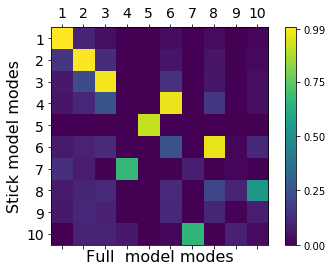
\includegraphics[width = .8\textwidth]{./Immagini/4_13.png}
	\caption{MAC colour matrix for the first ten modal shapes}
	\label{fig:4_8}
\end{figure}
A value of MAC $\approx 1$ means the modal shape of the \textit{i} mode of the full structure $\mathbf{\Phi_i}$  is similar to the modal shape of the \textit{j} mode of the stick structure $\mathbf{\Phi_j}$. \\
As we can see there is a large compatibility on the full bending modes, while the compatability of the torsional and coupled modes is lower.
\subsubsection{Frequencies Comparison}
As we said also a comparison on the first ten natural frequencies have been done. It's important to remark that the frequencies are ordered in ascending order by NASTRAN, so when the error on the frequencies is more than the step from two consecutive frequencies the frequency \textit{i} of the full model cannot be associated at the same mode of the frequency \textit{i} of the stick model. To avoid this problem it's required to order the frequencies using the modal shape order. To order the frequencies a visualization of the modal shapes is required, than we can recognize the type of the mode and associate the correct number to the mode to do the comparison.\\
In Fig. \ref{fig:4_9} there is the bar plot of the error between the full model natural frequencies and the stick model natural frequencies relative to the same modal shape:
\begin{figure}[H]
	\centering
	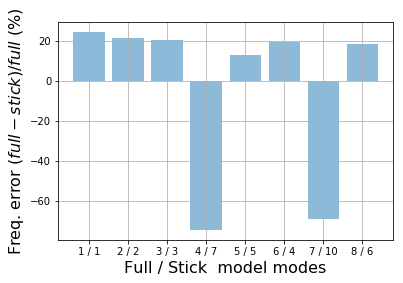
\includegraphics[width = .8\textwidth]{./Immagini/4_14.png}
	\caption{Bar plot of the error between the natural frequencies of the full and stick model}
	\label{fig:4_9}
\end{figure}
In Tab. \ref{tab:t1} there are the value of the first ten frequencies, ordered for the same modal shape for both model, and the relative error computed as:
\begin{equation*}
E= \frac{F_{i_{full}}- F_{i_{stick}}}{F_{i_{full}}}* 100
\end{equation*}
\begin{table}
\begin{tabular}{cccc}
	\toprule
	$Mode $  &  $Full\  model freq. [Hz]$  &  $Stick\  model freq. [Hz]$ & $Relative \ error [\%]$ \\
	\midrule
	$1$  &  $0.73553$  &  $0.55505$ & $ 24.53683 $\\
	$2$  &  $2.46789$  &  $1.92782$ & $ 21.88389 $\\
	$3$  &  $5.4666$  &  $4.33701$  &$  20.66340$\\
	$4$  &  $7.66535$  &  $13.3805$ &$ -74.55837 $  \\
	$5$  &  $9.40136$  &  $8.16675$  &$ 13.13220 $\\
	$6$  &  $9.50287$  &  $7.64263$  &$ 19.57560 $\\
	$7$  &  $13.2508$  &  $22.4217$  &$ -69.21020  $\\
	$8$  &  $14.4031$  &  $11.7250$  &$ 18.5939 $\\
	$9$  &  $19.613$  &  $21.4223$  &$ -9.22500 $\\
	$10$  &  $20.0155$  & $16.4092$ &$ 18.01750 $ \\
	\bottomrule
\end{tabular}
	\caption{Frequencies of full and stick model and relative error}
		\label{tab:t1}
\end{table} 
\section{Modification and Results}
As we can see the validation od the stick model is passed for the static analysis, while for the modal analysis there are some incompatibility. The modal shape related to the torsional and coupled torsional-bending modes are not quite similar, and the results on the natural frequencies present for this mode an error really high, and without sense. A modification at the stick model have been done to avoid this problem. After investigation we understand that the problems are related to the mass distribution, in fact while until the span wing there is a good discretization of the mass of the wing, 20 lumped muss are used, until the cord there isn't a valid distribution, all the lumped mass are positioned until the elastic axis, so the torsional behavior is not correctly represented. A new mass distribution have been implemented to correct this errors.
\subsection{New Mass Distribution}
As we showed in the first section to import the inertia proprieties of the full model on the stick model a series of lumped mass have been used. These lumped mass are positioned in the center of gravity of each box, that's mean that all the mass is concentrated until the elastic axis, then the torsional inertia proprieties of the full model are not imported in the stick model.\\
The idea to avoid this problem is to use a different mass distribution, in particular which takes into account of the distribution of mass until the cord. While just beam elements and lumped mass are used the only way to avoid this problem is to add lumped mass for each section and delocalise that mass from the elastic axis. \\
The new mass distribution provides to create 3 lumped mass for each box, one located in the trailing edge, one located in the center of gravity and one located in the leading edge. The value of the mass is chosen with a linear distribution on the cord, the total mass of the box should be unchanged. To do this the structure component have been modified, as first to compute the value of the 3 lumped mass, then to create the grid point to allocate the mass and finally to modify the \textit{.bdf} file. \\
\newpage
In Fig. \ref{fig:4_10} it's showed how the \textit{.dbf} file is built after the correction:
\begin{figure}[H]
	\centering
	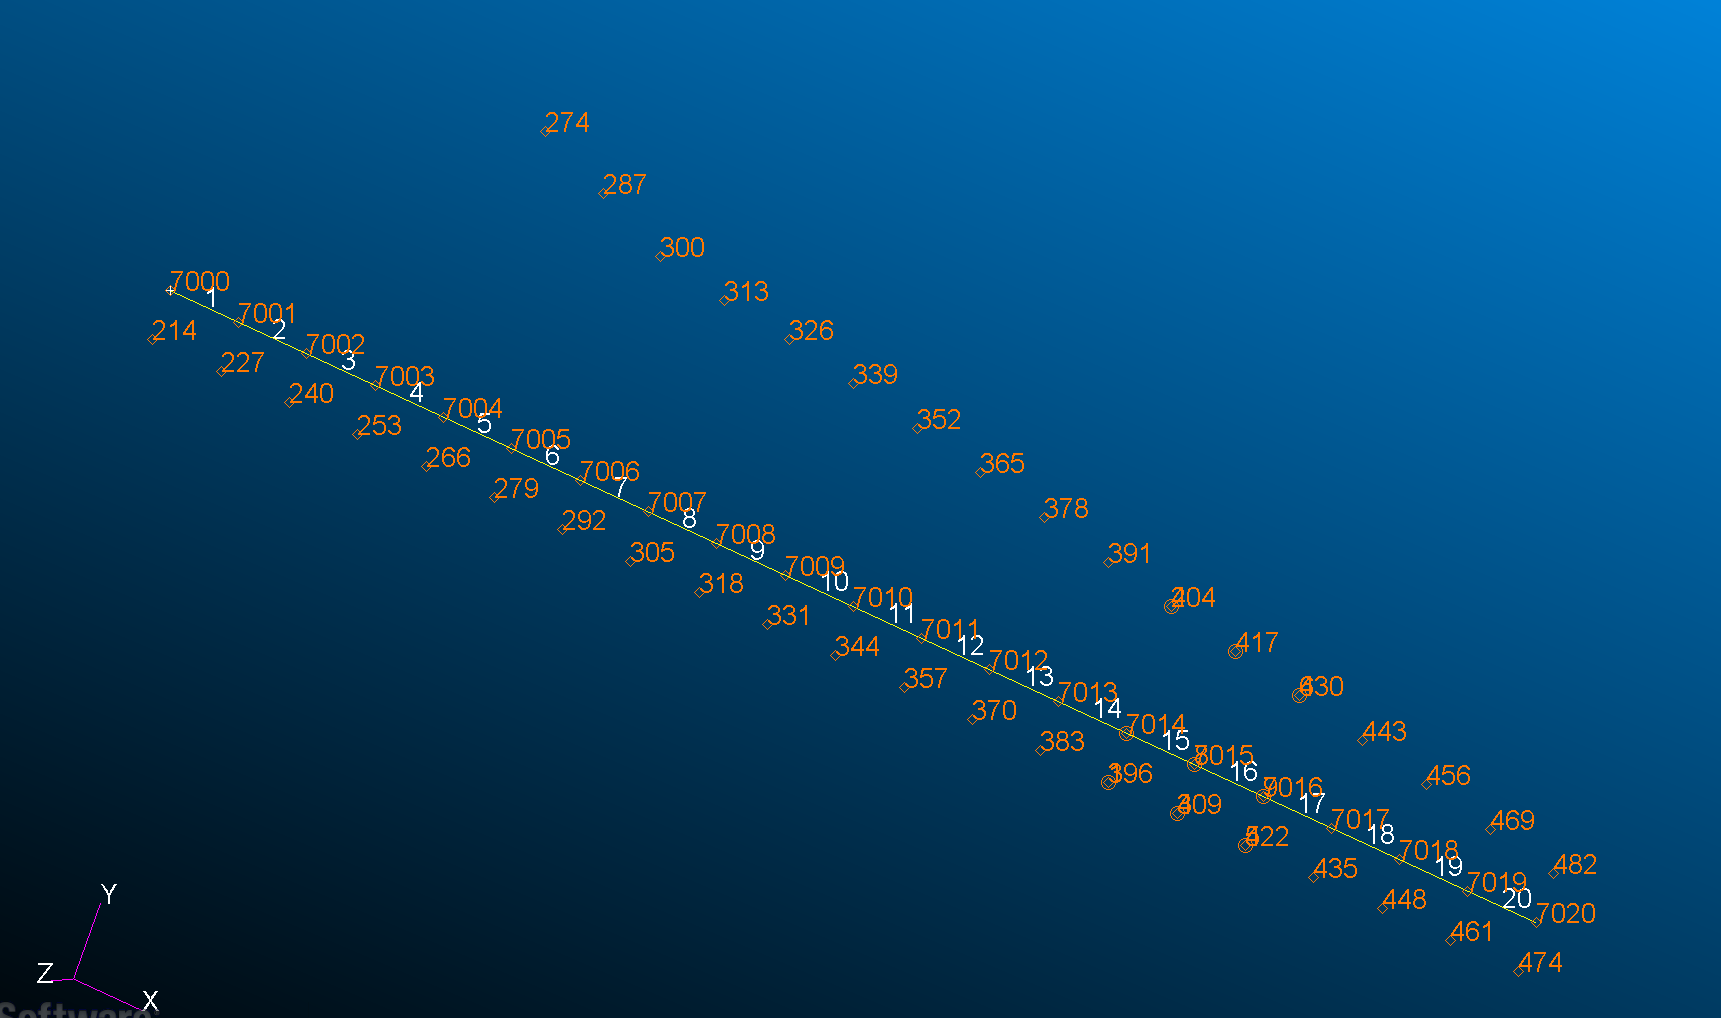
\includegraphics[width = 1\textwidth]{./Immagini/4_17.png}
	\caption{FEM model after new mass distribution implementation}
	\label{fig:4_10}
\end{figure}
In white there are the beam elements used for the stick model, in orange there are the lumped mass used, as u can see for each element, representative of one wing box section, there are 3 lumped mass, one localized on the center of gravity of the element, and two respectively localized on the trailing edge and on the leadng edge.\\
Using this new mass distribution as first we solved the problem related to the torsional modes, then the modal shapes and the frequencies related to the torsional and coupled mode assumed sense value, but there are also improvement on the bending modes. The error on the frequencies for the torsional and coupled mode are now of the same order of magnitude of the errors on the bending mode frequencies, and the last see a reduction of $\approx 5\%$.\\
\newpage 
The new MAC matrix and the new comparison between the frequencies are showed respectively in Fig. \ref{fig:4_11} and in Fig. \ref{fig:4_12}.
\begin{figure}[H]
	\centering
	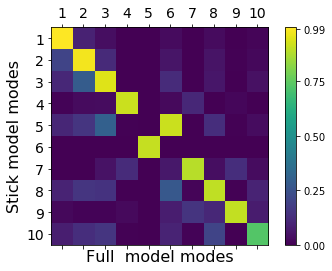
\includegraphics[width = .8\textwidth]{./Immagini/4_15.png}
	\caption{Improvements on the MAC matrix after correction}
	\label{fig:4_11}
\end{figure}
\begin{figure}[H]
	\centering
	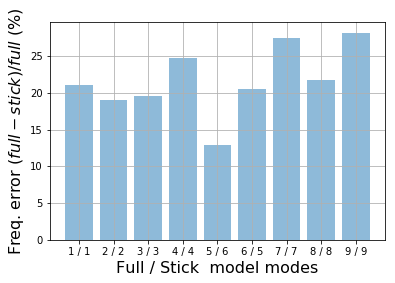
\includegraphics[width = .8\textwidth]{./Immagini/4_16.png}
	\caption{Improvements on the bar frequencies plot after correction}
	\label{fig:4_12}
\end{figure}
\newpage
In Tab. \ref{tab:t2} are showed the new frequencies for the stick model after correction and the relative errors:
\begin{table}
	\begin{tabular}{cccc}
		\toprule
		$Mode $  &  $Full\  model freq. [Hz]$  &  $Stick\  model freq. [Hz]$ & $Relative \ error [\%]$ \\
		\midrule
		$1$  &  $0.73553$  &  $0.55505$ & $ 21.0668$\\
		$2$  &  $2.46789$  &  $1.92782$ & $ 19.0021 $\\
		$3$  &  $5.4666$  &  $4.33701$  &$  19.6497$\\
		$4$  &  $7.66535$  &  $13.3805$ &$ 24.7905 $  \\
		$5$  &  $9.40136$  &  $8.16675$  &$ 12.9799 $\\
		$6$  &  $9.50287$  &  $7.64263$  &$ 20.6029 $\\
		$7$  &  $13.2508$  &  $22.4217$  &$ 27.5247   $\\
		$8$  &  $14.4031$  &  $11.7250$  &$21.778 $\\
		$9$  &  $19.613$  &  $21.4223$  &$28.2195  $\\
		$10$  &  $20.0155$  & $16.4092$ &$ 23.1296$ \\
		\bottomrule
	\end{tabular}
	\caption{Frequencies of full and stick model and relative error after correction}
	\label{tab:t2}
\end{table} 
\subsection{Automatization of the Mode Pairing }
Another problem of the reduction method was the non completely automatization of the process, that doesn't allow an implementation in the optimization process. In fact as we said, when the error on the frequencies is bigger than the step of two frequencies in the row, the order of the mode is not the same for the full and the stick model. Can happen that the 4th mode for the full model is the 1st torsional mode while for the stick model the 4th mode is the 3rd bending mode. Now for a correct evaluation of the errors on the frequencies and the relative correction the errors should be evaluate on the same mode, and the vector of frequencies need to be reorganized. This operation was did manually, by watching the modal shapes using a vizualization software for the output files. \\
To automatize the process we create an algorithm, based on the evaluation of the MAC matrix, to order the vector of frequencies related of the MAC value. In particular blocked the vector of the frequencies related to the full model, we put for each mode the frequencies related to the mode which have the maximum value of MAC, by exploring the full MAC matrix.\\
Once this function was implemented the reduction model could be implemented in the optimization loop to reduce the computational cost of the aeroelastic coupling loop.
\section{Results}
The main objective of this chapter is to prove that the stick model is reducing the overall time of the procedure and can be used for complex and multidisciplinary computations. Thus, in each component a timer was placed in order to calculate the time reduction of the stick model. Certainly, in the first iterations the advantage of the stick model will not be evident since there are two additional components in comparison with the 3D model, thus, extra time. However, when the process reaches the multidisciplinary analysis(MDA), the computational efficiency of the stick model should be clear. \cite{bru}\\
In Tab. \ref{tab:t3} the time cost of each component in both optimizations are presented:
\begin{table}
	\begin{tabular}{l|rr|r}
		\toprule
		$Component $  &  $Full\  model [s]$  &  $Stick\  model [s]$ & $Reduction [\%]$ \\
		\midrule
		$Geometry$  &  $7.97$  &  $7.81$ & $ -2.01$\\
		$Interpolation$  &  $0.371$  &  $0.416$ & $ -88.79 $\\
		$Total\  Reduction$  &  $-$  &  $7.27$  &$  -$\\
		$Aero$  &  $7.26$  &  $7.25$ &$ -0.28$  \\
		$Load\  Transfer$  &  $0.0044$  &  $0.00183$  &$ -58.41 $\\
		$Structure$  &  $3.52$  &  $2.19$  &$ -37.78$\\
		$Displacements \ Transfer$  &  $0.00166$  &  $0.000605$  &$ -63.55   $\\
		$Total\ Pre-MDA \ Process$  &  $8.341$  &  $15.1216$  &$81.29 $\\
		$Total\ MDA\ Process$  &  $10.78606$  &  $9.432435$  &$-12.55  $\\
		$Total\ Time$  &  $116.2016$  & $107.7537$ &$-7.27$ \\
		\bottomrule
	\end{tabular}
	\caption{Time reduction of the stick model}
	\label{tab:t3}
\end{table} 







